\subsubsection{Metrics Engine}
\label{metricsengine}
The core of the open framework is the ecosystem \gls{graphite} (\glsdesc{graphite}), which captures performance values over time. 
Started in 2006 it provides a modular system to consume, process, store and access metric information in the form \texttt{key value timestamp}.

The metrics are persisted in round-robin databases using the \texttt{whisper} format by a set of daemons called \texttt{carbon}.
\autoref{lst:carbon_wsp} shows an example of how performance metrics are processed and stored.

\begin{lstlisting}[language=bash,
    caption={Sending metric strings \texttt{test.metric <value> <timestamp>} via \texttt{netcat} (short \texttt{nc}) to the carbon daemon (port \texttt{2003}). Afterward reading the \texttt{timestamp, value} pairs for the specific \texttt{whisper} file.},
    label={lst:carbon_wsp}]
$ for x in {1..5};do
> echo "test.metric ${x} $(date +%s)" |\
    nc -w 1 127.0.0.1 2003
> sleep 5
> done
$ export CDIR=/var/lib/carbon/whisper
$ whisper-fetch $CDIR/test/metric.wsp |\
    grep -v None
1438513460	1.000000
1438513465	2.000000
1438513470	3.000000
1438513475	4.000000
1438513480	5.000000
$
\end{lstlisting}

The \gls{graphite} framework provides a rich ecosystem of visualizations (the default metrics WebUI is shown in \autoref{fig:graphite_web}, plugins, metric sources and alternative daemon implementation to fit almost
all use-cases around metrics gathering, processing, storing and serving. Due to its open-source development and stable API, missing pieces
can be added if needed.

\begin{figure}[!ht]
    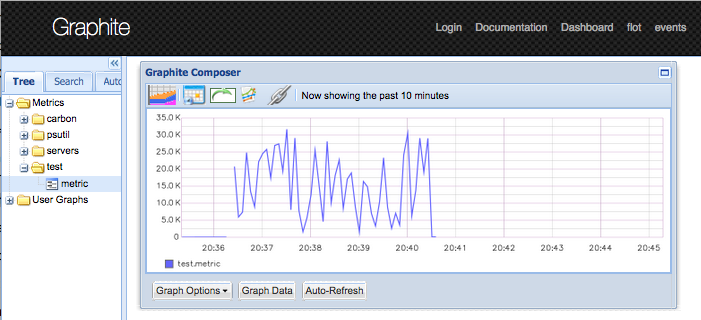
\includegraphics[width=.4\textwidth]{images/png/graphite_web.png}
    \caption{\label{fig:graphite_web}Example of a plain visualization of metrics using the default WebUI which is provided by the \gls{graphite} ecosystem from the beginning.}
\end{figure}

This enables each part of the infrastructure layer to submit metrics without much effort. Even application developers can just start sending metrics down the pipeline and
trust that the metrics will be available at the user interface once they are processed.

\subsubsection{Metric Key Scheme}

If the group of metric generators grows to a certain complexity, the metric keys become a problem, since naming schemes vary depending on the context of
the producer. An engineer overseeing the network in a data-center might organize his/her metrics hierarchically (\lstinline{datacenter01.rack01.compute01.eth0.send_bytes}), while from the
resource scheduler perspective a grouping per job (\lstinline{jobid01.compute01.send_bytes}) is a scheme which might fit the use-case best.

To overcome this issue a scheme should be chosen which abstracts from a metric key as single string.
The Metrics2.0\footnote{\Mundus~\url{http://metrics20.org/}} idea (an example is shown in \autoref{lst:metrics20}) is to annotate metrics with metadata.

\begin{lstlisting}[language=bash,
    caption={Metrics2.0 formatted metric},
    label={lst:metrics20}]
{
    server: dfs1
    what: diskspace
    mountpoint: srv/node/dfs10
    unit: B
    type: used
    metric_type: gauge
    value: 1024
}
meta: {
    agent: diamond,
    processed_by: statsd2
}
\end{lstlisting}

\subsubsection{Grafana}
As the name might suggest Grafana uses the framework of Kibana (see Section~\ref{kibana}),
but is intended to visualize metrics using the \gls{graphite} API,
hence the name which combines the two words (\textbf{Gra}phite + \textbf{f} + Ki\textbf{bana}).
Even though it originated as pure metric visualization tool, it allows to annotate syslog events stored in an Elasticsearch instance (due to its origins a simple task).
Furthermore Grafana is able to query other data back-ends than Graphite, namely \gls{tsdb}\glsdesc{tsdb} and \gls{influxdb}\glsdesc{influxdb}.